\subsection{Nearly Sorted Data}
\subsubsection{Time}
Execution time unit: milliseconds
\begin{table}[h!]
\centering
\begin{tabular}{|l|r|r|r|r|r|r|}
\hline
\textbf{Algorithm} & \textbf{10000} & \textbf{30000} & \textbf{50000} & \textbf{100000} & \textbf{300000} & \textbf{500000} \\
\hline
Selection Sort & 83.898 & 754.469 & 2097.2 & 8461.66 & 76561.9 & 210139 \\ \hline
Insertion Sort & 0.02 & 0.0912 & 0.0799 & 0.1037 & 0.1879 & 0.3103 \\ \hline
Shell Sort & 20.4246 & 195.299 & 484.834 & 1795.67 & 15977.1 & 49089.4 \\ \hline
Bubble Sort & 14.3526 & 124.481 & 347.676 & 1339.36 & 12296.1 & 34055 \\ \hline
Heap Sort & 0.6889 & 2.3363 & 3.8533 & 8.278 & 29.1528 & 43.6957 \\ \hline
Merge Sort & 2.497 & 8.2457 & 12.1077 & 27.873 & 72.59 & 120.094 \\ \hline
Quick Sort & 19.2834 & 152.439 & 1281.55 & 7068.34 & 68668.4 & 197042 \\ \hline
Radix Sort & 0.1272 & 0.5591 & 0.8446 & 1.5646 & 5.8751 & 10.27 \\ \hline
Counting Sort & 0.0155 & 0.043 & 0.0714 & 0.1567 & 0.7502 & 1.4829 \\ \hline
Binary Insertion Sort & 0.271 & 0.9111 & 1.4968 & 3.1023 & 9.2867 & 16.3849 \\ \hline
Shaker Sort & 0.1591 & 0.3401 & 0.2698 & 0.327 & 0.3967 & 0.5661 \\ \hline
Flash Sort & 0.0961 & 0.3437 & 0.6098 & 0.992 & 4.0775 & 6.7901 \\
\hline
\end{tabular}
\label{table:nearly_sorted_execution_time}
\end{table}

\begin{figure}[h]
    \centering
    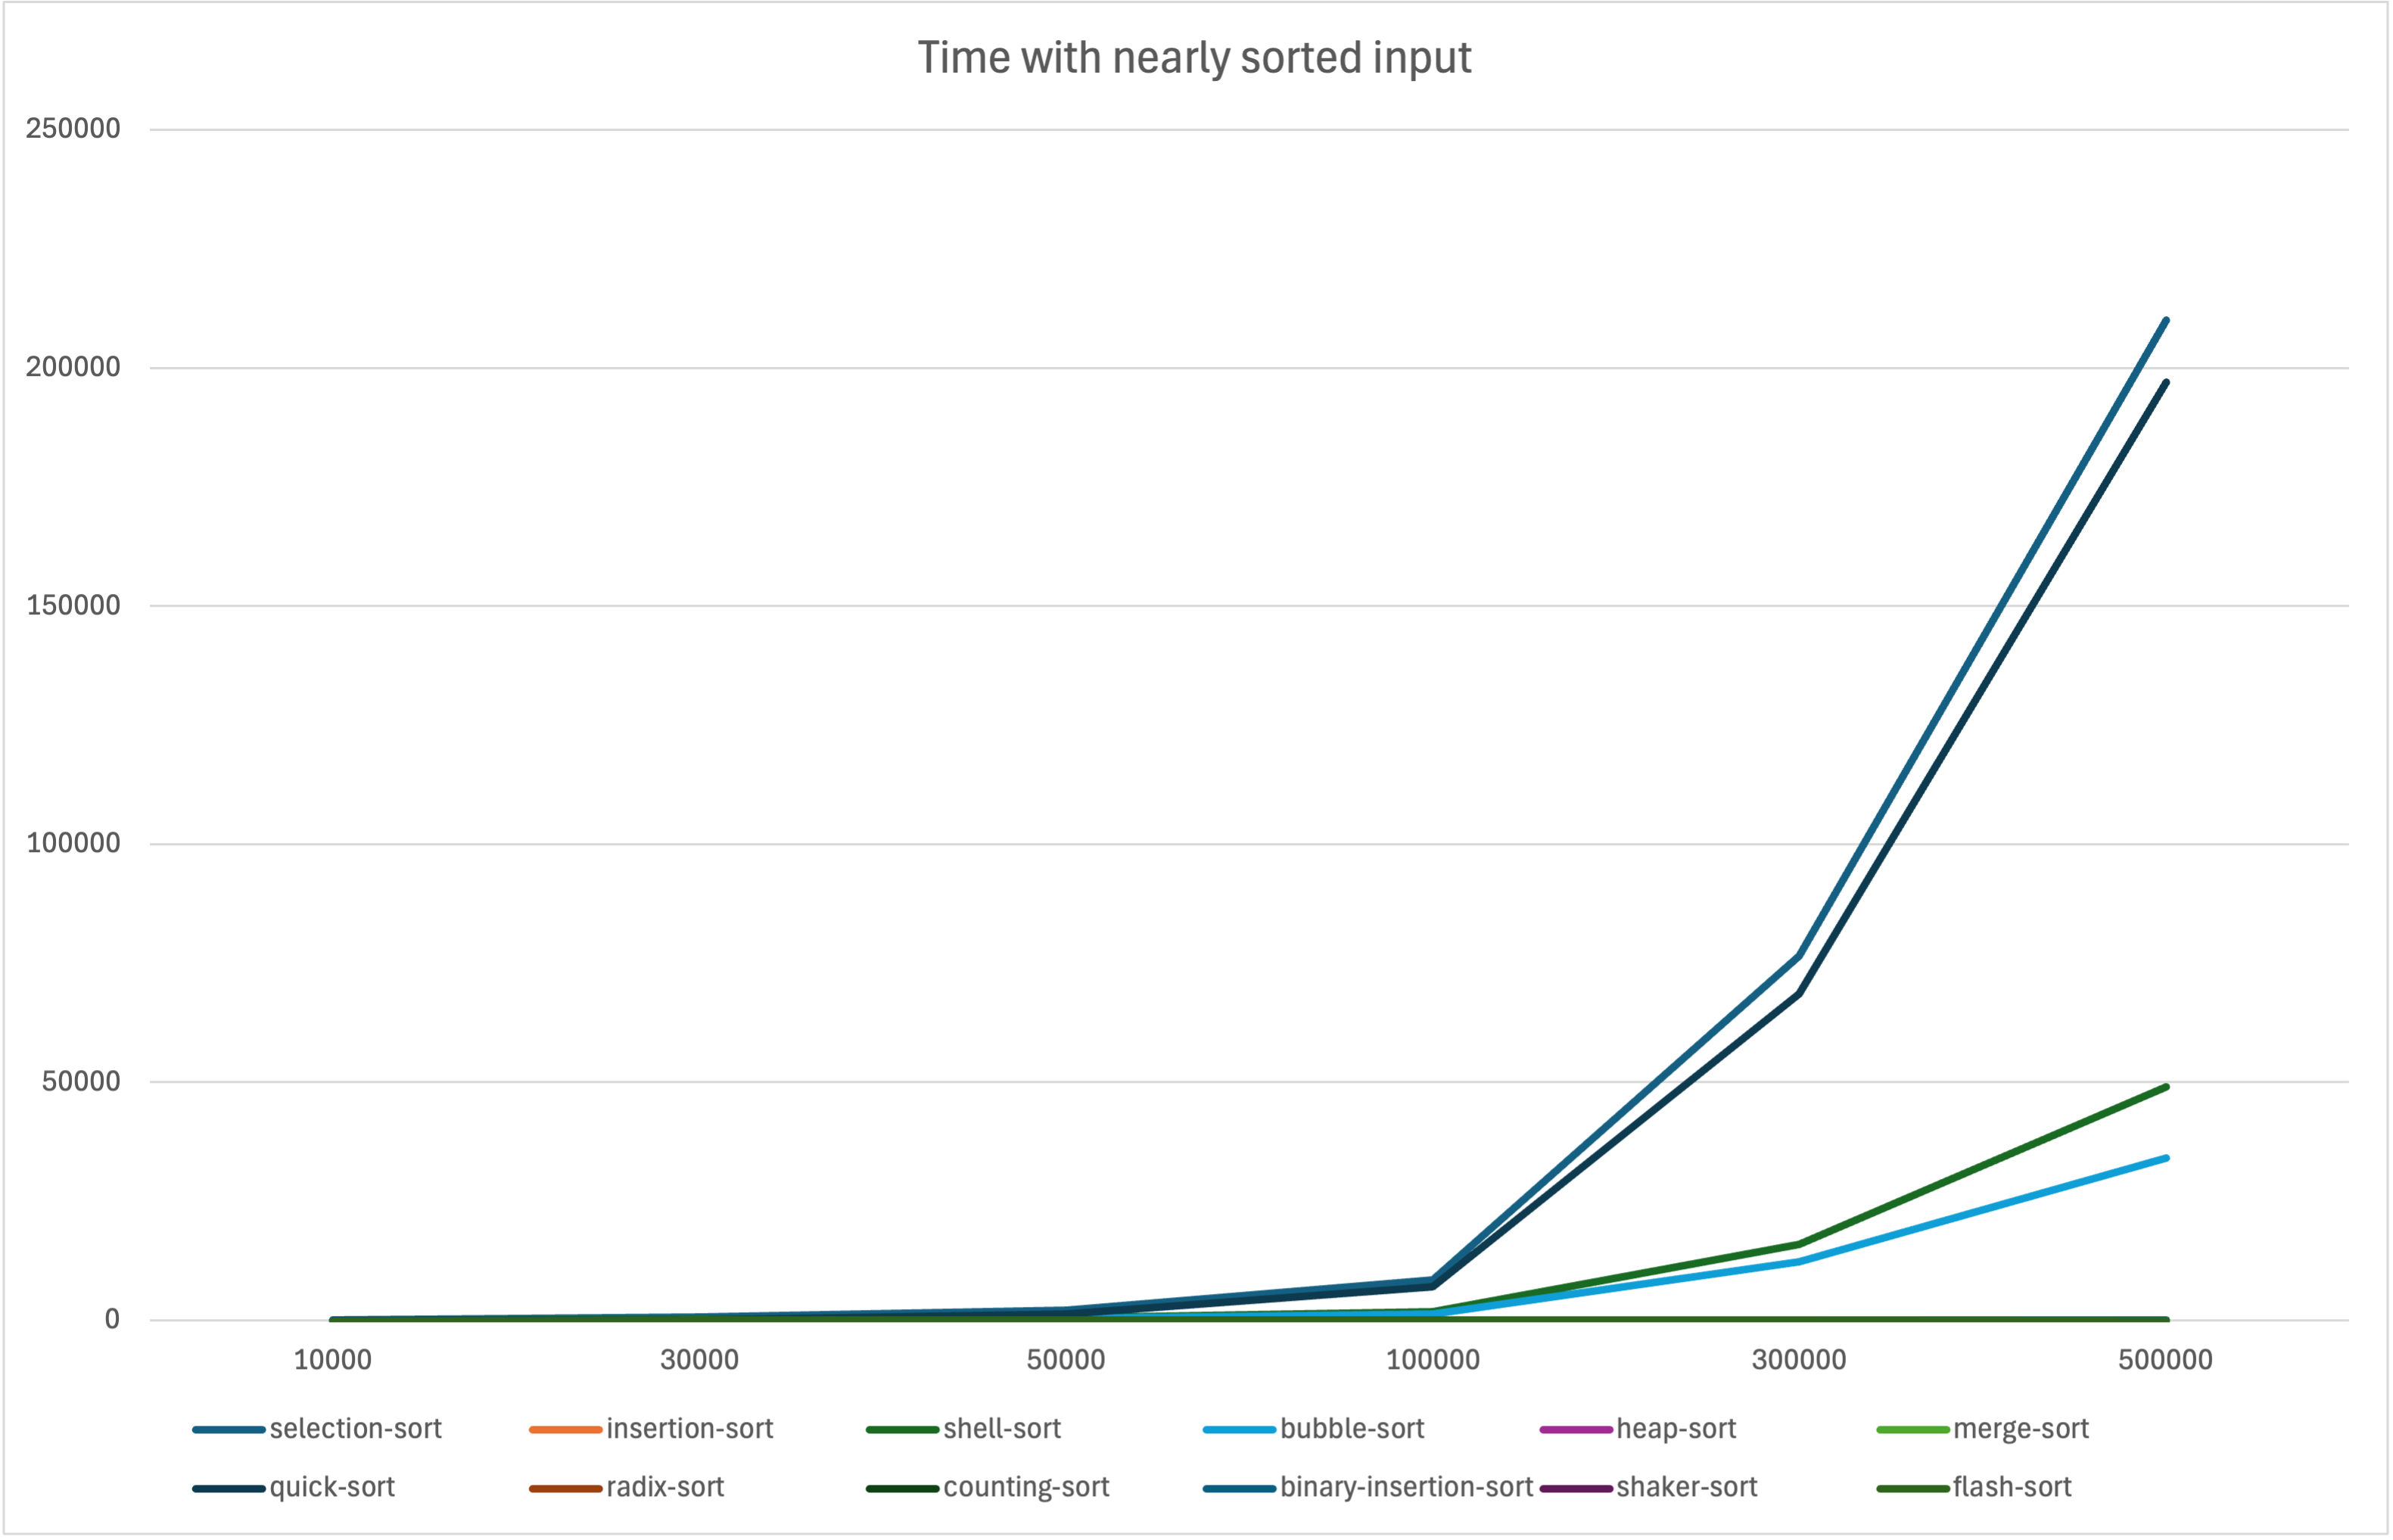
\includegraphics[scale=.65]{Figures/Visualization/Nearly_time.png}
    \caption{Execution time for Nearly Sorted data}
    \label{fig:enter-label}
\end{figure}

\textbf{Comments on the running time of sorting algorithms with nearly sorted data}

\begin{enumerate}
    \item \textbf{Fastest Algorithm:} \\
  - For small data sizes (10,000 - 50,000), \textit{Insertion Sort} has the fastest execution time. \\
  - As data size increases (100,000 - 500,000), \textit{Counting Sort} and \textit{Flash Sort} become the most efficient in terms of execution time.

    \item \textbf{Slowest Algorithm:}
  - \textit{Selection Sort} and \textit{Bubble Sort} are the slowest algorithms for all data sizes.

    \item \textbf{General Comments:}
  - Algorithms like \textit{Quick Sort}, \textit{Merge Sort}, and \textit{Heap Sort} have moderate execution times, better than \textit{Selection Sort} and \textit{Bubble Sort}, but slower than \textit{Counting Sort} and \textit{Flash Sort}.
\end{enumerate}


\subsubsection{Comparison}
\begin{table}[h!]
\centering
\begin{tabular}{|l|r|r|r|r|r|r|}
\hline
\textbf{Algorithm} & \textbf{10000} & \textbf{30000} & \textbf{50000} & \textbf{100000} & \textbf{300000} & \textbf{500000} \\
\hline
Selection Sort & 100020001 & 900060001 & 2500100001 & 10000200001 & 90000600001 & 2.50001E+11 \\ \hline
Insertion Sort & 147654 & 744478 & 651114 & 801114 & 1401114 & 2069258 \\ \hline
Shell Sort & 136486703 & 1228074234 & 3411144570 & 13643867417 & 1.2279E+11 & 3.41082E+11 \\ \hline
Bubble Sort & 100009999 & 900029999 & 2500049999 & 10000099999 & 90000299999 & 2.5E+11 \\ \hline
Heap Sort & 669993 & 2236691 & 3925392 & 8364913 & 27413230 & 47404908 \\ \hline
Merge Sort & 507409 & 1666255 & 2833852 & 5856684 & 18744620 & 32121800 \\ \hline
Quick Sort & 29623224 & 252918102 & 1706786888 & 9235419190 & 89219734904 & 2.49335E+11 \\ \hline
Radix Sort & 140051 & 510064 & 850064 & 1700064 & 6000077 & 10000077 \\ \hline
Counting Sort & 60003 & 180003 & 300003 & 600003 & 1800003 & 3000003 \\ \hline
Binary Insertion Sort & 437075 & 1467163 & 2451861 & 4879730 & 15700082 & 27071229 \\ \hline
Shaker Sort & 183347 & 474192 & 465899 & 565899 & 965899 & 1475760 \\ \hline
Flash Sort & 118975 & 356977 & 594976 & 1189973 & 3569971 & 5949978 \\
\hline
\end{tabular}
\label{table:nearly_sorted_number_of_comparisons}
\end{table}

\begin{figure}[h]
    \centering
    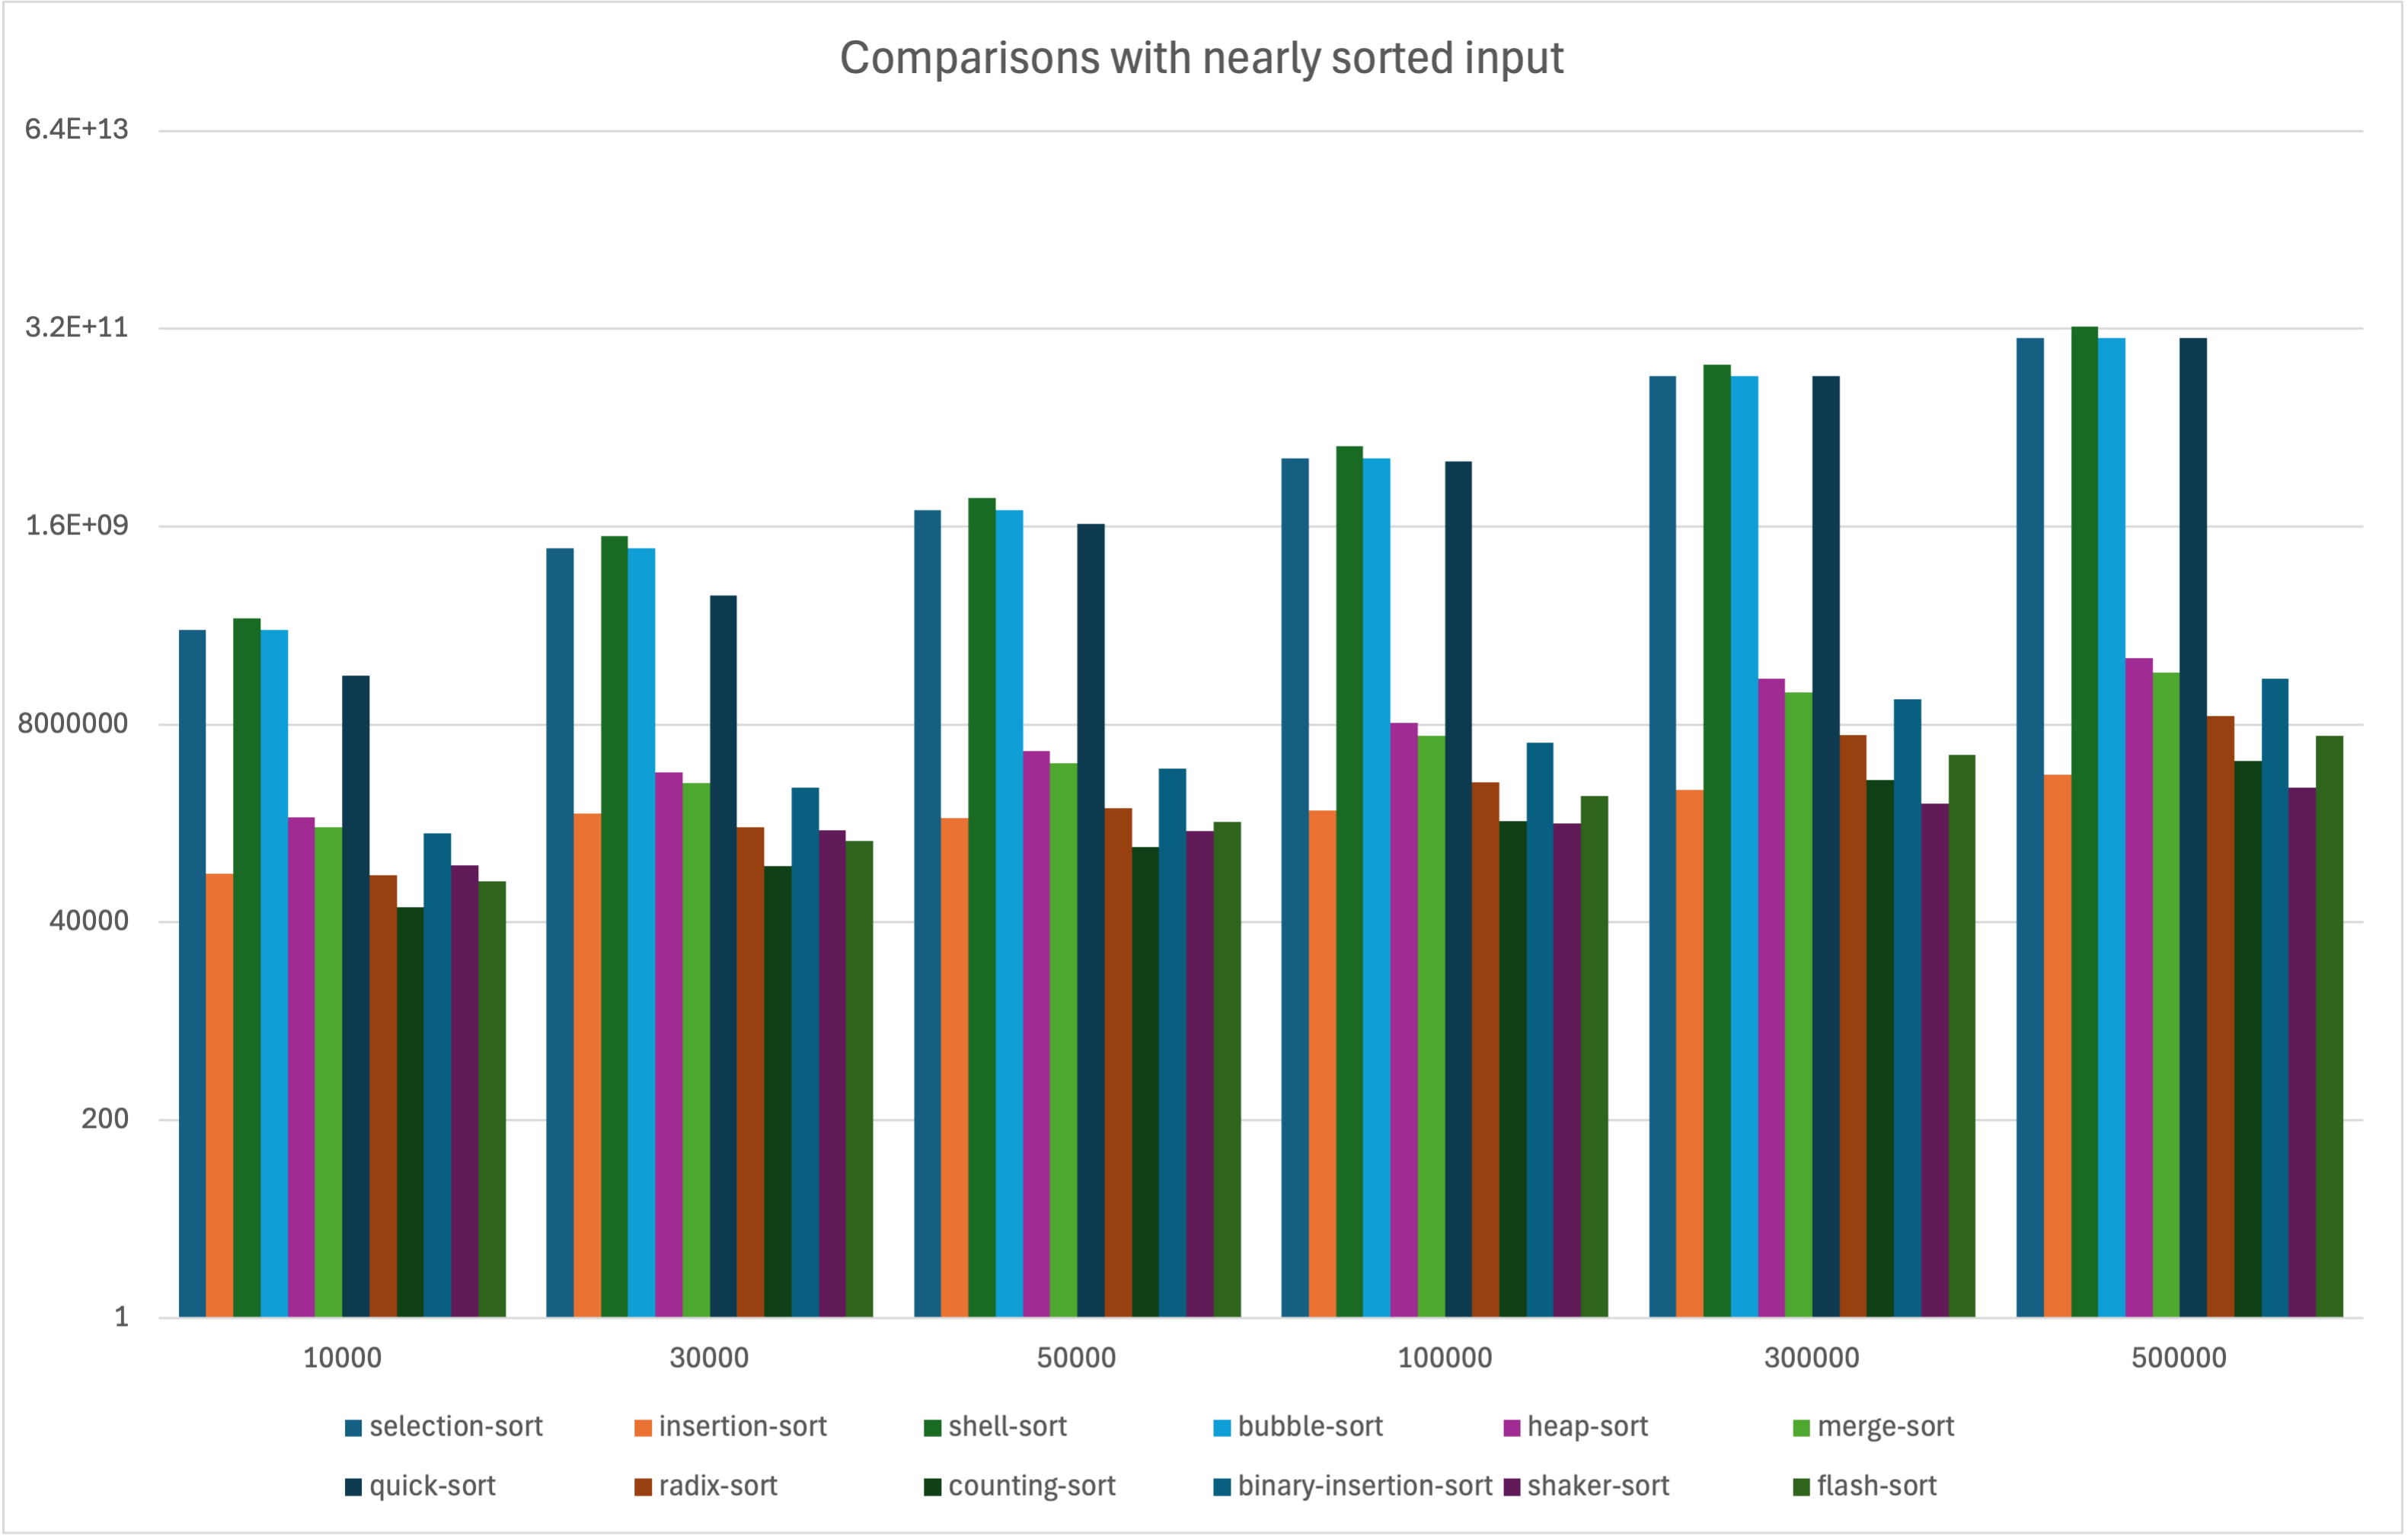
\includegraphics[scale=.65]{Figures/Visualization/Nearly_compare.png}
    \caption{Number of comparisons of the algorithm for Nearly Sorted data}
    \label{fig:enter-label}
\end{figure}

\textbf{Comments on the number of comparisons of sorting algorithms with nearly sorted data}

\begin{enumerate}
    \item \textbf{Algorithm with Fewest Comparisons:} \\
  - \textit{Counting Sort} and \textit{Radix Sort} have the fewest comparisons for all data sizes.

    \item \textbf{Algorithm with Most Comparisons:}
  - \textit{Selection Sort}, \textit{Bubble Sort}, and \textit{Shell Sort} have the most comparisons for all data sizes.

    \item \textbf{General Comments:} \\
  - Algorithms like \textit{Merge Sort} and \textit{Heap Sort} have relatively fewer comparisons compared to \textit{Selection Sort} and \textit{Bubble Sort}.
\end{enumerate}

\subsubsection{Overall}
\begin{enumerate}
    \item \textbf{By Data Order:}
    \begin{itemize}[label=-]
        \item  \textit{Insertion Sort} performs best when the data is nearly sorted.
        \item \textit{Selection Sort} and \textit{Bubble Sort} remain slow and inefficient with nearly sorted data.
    \end{itemize}
    
    \item \textbf{By Data Size:}
    \begin{itemize}[label=-]
        \item  For small data sizes, \textit{Insertion Sort} and \textit{Counting Sort} have the best execution times.
        \item  For large data sizes, \textit{Counting Sort} and \textit{Flash Sort} excel in execution time.
        \item \textit{Quick Sort} and \textit{Merge Sort} can be considered good choices for medium to large data sizes due to their balance between execution time and comparison count.
    \end{itemize}
    
    \item \textbf{Grouping Stable/Unstable Algorithms:}
    \begin{itemize}[label=-]
        \item  \textbf{Stable:} \\
  - \textit{Insertion Sort}, \textit{Merge Sort}, and \textit{Binary Insertion Sort} are stable algorithms, ensuring the order of equal elements is preserved.
  
        \item  \textbf{Unstable:} \\
  - \textit{Quick Sort}, \textit{Heap Sort}, and \textit{Shell Sort} are unstable algorithms and may change the order of equal elements.
    \end{itemize}
\end{enumerate}